\chapter{Automaton}

%%%%%%%%%%%%%%%%%%%%%%%%%%%%%%%%%%%%%%%%%%%%%%%%%%%%%%%%%%%%%%%%%%%%%%%%%%%%%
\section{Definition and Representation of an Automaton}
A finite automaton is a Finite State System composed of discrete inputs and outputs. It is a mathematical model of system composed of a finite number of states. Each state summarize informations and the configuration of these states determine the behavior of the system. We could for example model a human brain with a finite state system considering that each neuron contains informations which can be described by a small number of bits. Furthermore the number of neurons is limited to $2^{35}$ at most.\\
We consider an automaton as a set of states and transitions from state to state that occur on input symbols. We can model the system as a graph, called a \textit{transition diagram} which is associated with a finite automaton. The verticals of the graph correspond to the states of the finite automaton. Each state is modeled by an unique circle labeled and transitions are modeled by an arrow from one state to another one that is also labeled. An event can occur many times but a state is unique.\\
This definition is inspired by the book \textit{introduction Automata Theory Langage and Computation} written by John E Hopcroft, R.Motwani and Jeffrey D.Ullman. \cite{introductionAutomataTheoryLangageComputation_2007}\\

\subsubsection*{For example : A light}
We model a light that starts and switch on off if one press the button :
\begin{center}
      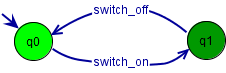
\includegraphics[width = 5cm]{./IV/ex1.png}
      \captionof{figure}{\label{automate}Example 1 - finite automaton}
      \vspace{0.5cm}
\end{center}

This automaton is composed of :
\begin{itemize}
\item two states : {q0,q1}
\item an initial state : {q0}
\item two transitions : {switch\_off, switch\_on}
\end{itemize}

In a maze context, objects and the dynamics walls have a behavior we can model with automaton. The object moves can have as possible transitions $up$, $down$, $left$, $right$, the walls can also have moves, $up$, $down$, $left$, $right$. Each cell of our maze is a state where few events can occur. For example, each possible event that can happen on every cell - if we don't know the position of the object - is described by the next automaton \ref{maze} :

\begin{figure}[H]
\begin{minipage}{0.5 \textwidth}	
      \begin{center}
      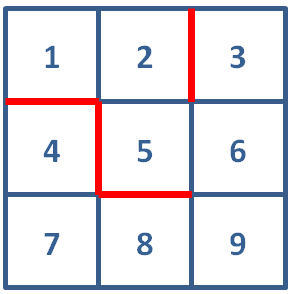
\includegraphics[width = 3cm]{./IV/3x3lab.png}
      \caption{Example - Maze}
      \end{center}
\end{minipage}
\begin{minipage}{0.5 \textwidth}
\begin{center}
      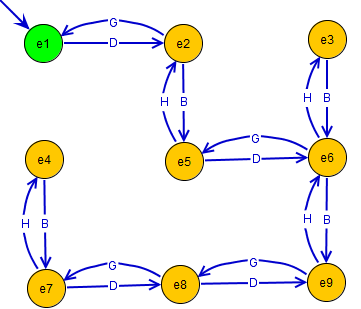
\includegraphics[width = 4cm]{./IV/3x3autom.png}
      \captionof{figure}{\label{maze} Example - Automaton }
      \end{center}
\end{minipage}
\end{figure}


\section{Formal representation of an deterministic automaton}
We formally denote a finite automaton by the next 5-tuple :
\begin{equation}
\mathcal{A} = ( Q, \Sigma,\delta,q_0,F )
\end{equation}

With :

\begin{tabular}{lll}
$Q$ & : & finite set of states.\\
$\Sigma$ & :& finite input alphabet.\\
$q_0$ & :& $q_0 \in Q$ the initial state.\\
$F$ & :& $F \subset Q$ the set of final states\\
$\delta$ & :& the transition function mapping $Q$ x $\Sigma$ to $Q$
\end{tabular}\\
\begin{description}
\item [Alphabet :] set of all events known by the automaton
\item [String :] one sequence of transitions
\item [The transition function :] a string x is accepted by the automaton $\mathcal{A}$  if $\delta(q_0,x)=p$
\end{description}


%%%%%%%%%%%%%%%%%%%%%%%%%%%%%%%%%%%%%%%%%%%%%%%%%%
%Rajouter ref vers la bliblio
\section{Formal representation of a nondeterministic automaton}
As explained by Hopcroft, Motwani and Ullman \cite{introductionAutomataTheoryLangageComputation_2007}, \textit{"a nondeterministic automaton has the power to be in several states at once"}. In the formalization we supposed that a same input can arrive to several states. The definition of an automaton remains mainly the same.
\begin{equation}
\mathcal{A} = ( Q, \Sigma,\delta,q_0,F )
\end{equation}

With :

\begin{tabular}{lll}
$Q$ & : & finite set of states.\\
$\Sigma$ & :& finite set of input alphabet.\\
$q_0$ & :& $q_0 \in Q$ the initial state.\\
$F$ & :& $F \subset Q$ the set of final states\\
$\delta$ & :& the transition function mapping $Q$ x $\Sigma$ to $\mathcal{P}(Q)$
\end{tabular}\\

The difference between a nondeterministic and a deterministic automaton is the type of value that $\delta$ returns. Thus, the transition function is extended : \\
\begin{equation*}
w=xa
\end{equation*} where $a$ is the final letter of $w$ and $x$ is the rest of $w$
\begin{equation*}
\widehat{\delta}(q,x)=\{p_1,p_2,...,p_k\}
\end{equation*}
\begin{equation*}
\bigcup_{k}^{i=1}\delta(p_i,a) = \{r_1,r_2,...,r_m\}
\end{equation*}
Then \begin{equation*}
\widehat{\delta}(q,w) = \{r_1,r_2,...,r_m\}
\end{equation*}

Cassandras define nondeterministic finite automata as \cite{cassandras2009introduction}:
\begin{equation*}
\widehat{\delta} : Q × \Sigma \rightarrow 2^X
\end{equation*}
\begin{equation*}
\widehat{\delta}(x, s) \subseteq Q
\end{equation*}
with
\begin{equation*}
q_0 \subseteq Q.
\end{equation*}

\subsection{Language Notation and Definitions}
Definition (Language and notation, \cite{cassandras2009introduction})  : A language defined over an event set $L$ is a set of finite-lenght strings formed from events in E.\\
As an example, let $\Sigma=\{a, b, g\}$ be the set of events. We define a language :
$L=\{\epsilon, a, abb\}$.\\
The definition of the language for an automaton is really useful to analyze it. Language is a mathematical tool used to do operations, in order to extract many properties for automata. We recall how to express the language of an automaton then the operations below.

%%%%%%%%%%%%%%%%%%%%%%%%%%%%%%%%%%%%%%%%%%%%%%%%%%%%%%
\subsection{Languages Represented by Automata}
Definition by Cassandras\cite{cassandras2009introduction} :\\
The language generated by $ A = ( Q, \Sigma,\delta,q_0,F )$ is :
\begin{equation*}
\mathcal{L}(A) := \{ s \in \Sigma^* \delta(q_0,s) \text[is \hspace{0.1cm} defined] \}
\end{equation*}


The language marked by $A$ is :
\begin{equation}
\mathcal{L}_m(A) := \{ s \in \mathcal{L}(A) : \delta(q_0, s) \in F\}
\end{equation}
with the extended transition function : $\delta : Q$ × $\Sigma ^{∗} \rightarrow F $ with $\epsilon \in \mathcal{L}(A)$\\

%Lien entre language et automates
The language generated by $A$ represents all strings existing in the automaton starting at the initial state. The string is the concatenation of the event labels of the transitions for a path in an automaton. It is also called a sequence.\\
The marked language represents all strings ending at a marked state. We also said that the language is \textit{recognized} by the automaton.

\textbf{\underline{For instance :}} \\
      \begin{center}
      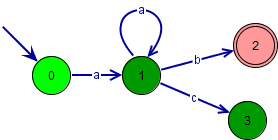
\includegraphics[width = 5cm]{./IV/ex2.png}
      \captionof{figure}{Automaton example}
      \end{center}
      
This finite state automaton is $\mathcal{A} = (Q, \Sigma,\delta,q_0,F )$  with :
\begin{itemize}
\item $Q=\{0,1\}$
\item $\sigma = \{a,b,c\}$
\item $q_0 = {0} $
\item $F=\{2\}$
\item $\delta(0,a)=1$, $\delta(1,a)=1$, $\delta(1,b)=2$, $\delta(1,c)=3$
\end{itemize}

We can see from the figure and the definitions that :
\begin{itemize}
\item $\mathcal{L}_m (A)=aa*b$
\item $\mathcal{L}_g (A)=aa*(b+c)$
\end{itemize}


% \begin{equation*}
% \mathcal{L}(G) = \{s \in E^* : (\exists q \in q_0) [\delta(q, s) \text[is\hspace{0.1cm}defined] ]\}
% \end{equation*}
% \begin{equation*}
% \mathcal{L}(G) = \{s \in \mathcal{L}(G) : (\exists q \in q_0)[\delta(q, s) \cap F = \emptyset]\}
% \end{equation*}

We formally define the language for a deterministic automaton as :\\
\begin{equation*}
L(\mathcal{A}) = \{x|\delta(q_0,x) \cap F\}
\end{equation*}

if a state is accepted by the one finite automaton, it is a \textit{regular set} \\
\\
The language accepted by the nondeterministic finite automaton is defined by : 
\begin{equation*}
L(\mathcal{A}) = \{w|\widehat{\delta}(q_0,x)\} \cap F \neq \emptyset
\end{equation*}
If a main sequence of choices from a start state to any accepting state if possible, it accepts a string $w$ .

%%%%%%%%%%%%%%%%%%%%%%%%%%%%%%%%%%%%%%%%%%%%%%%%%%%%%%%%%%%%%%%%%%%%
\subsection{Operations} 

Let's consider two languages L and M.\\
\begin{description}
\item [Union] : $L \cup M$ set of strings which are in the languages L or M
\item [Concatenation] : the concatenation of L and M is detoned by a "dot" or nothing as $L.M$ or $LM$. LM contains each string in L concatenated with each string in M. Each string must only appear once. The empty string $\epsilon$ is the identity element : $u \epsilon = \epsilon u = u$
\end{description}
\begin{equation*}
L,M \subseteq E^*
\end{equation*}
\begin{equation*}
LM := \{s \in E^*: (s = s_Ls_M) and (s_L ∈ La) and (s_M \in L_M)\}
\end{equation*}

\begin{description}
\item [Kleene-closure/ Kleene star] : it is denoted $L^*$, any number of possible strings  with repetitions, concatenating all, including the empty string $\epsilon$.
\end{description}
\begin{equation*}
L \subseteq E^*
\end{equation*}
\begin{equation*}
L^∗ := {\in} \cup L \cup LL \cup LLL \cup ...
\end{equation*}

\begin{description}
\item [Projection] : 
\end{description}

\begin{equation*}
L \subseteq E_l^*
\end{equation*}
\begin{equation*}
P(L) :=\{ t \in E_s^* : (\exists \in L) [P(s)=t] \}
\end{equation*}

\begin{equation*}
L \subseteq E_s^*
\end{equation*}
\begin{equation*}
P^{-1}(L_s) := \{ s \in E_l^* : (\exists t \in L_s) [P(s)=t] \}
\end{equation*}

\begin{description}
\item [Example of operations for Languages] : $E=\{a,b\}$ and $L =\{c, acb, abc, cacacb, aacbcab\}$
\item\hspace{6.6cm} Consider the projection : $ P: E_l^* \rightarrow E^*$\\
\end{description}

\begin{center}
$P(L) = \{ \epsilon, ab, aab, aabab\}$ \\
$P^{-1}(\{\epsilon\}) = \{c\}^*$\\
$P^{-1}(\{b\}) = \{c\}^*{b}{c}*$
\end{center}



%%%%%%%%%%%%%%%%%%%%%%%%%%%%%%%%%%%%%%%%%%%%%%%%%%%%%%%%%%%%%%%%%%%%%%%%%
\subsection{Properties}
The properties below were extracted by the operations.
\begin{description}
\item [Language-equivalent automata \cite{cassandras2009introduction} ] : Automata G1 and G2 are said to be language-equivalent if
$\mathcal{L}(G_1) = \mathcal{L}(G_2)$ and $\mathcal{L}_m(G_1) = \mathcal{L}_m(G_2)$ \\

\item [Blocking] : Automaton G is said to be blocking if $ \mathcal{L}_m(G_1) \subset\mathcal{L}(G) $
and nonblocking when $ \mathcal{L}_m(G_1) \subset \mathcal{L}(G) $

\item [Accessibility] : A state is said $accessible$ a sequence/word exists from the initial state to this state. With the definition $\mathcal{L}(G)$ and $\mathcal{L}_m(G)$ explained above, we can apply them to find all existing words from the initial state to all reachable states :
\end{description}


\begin{equation*}
A_{ac} = \{q \in Q | (\exists s \in \Sigma^∗) [\delta(q_0, s) = q]\}
\end{equation*}

\vspace{0.5cm}

An automaton is defined as $accessible$ if all its states are accessible : $Ac(A)=Q$.\\
Despite as it is explained in \cite{cassandras2009introduction} by \textit{Cassandras and Lafortune}, we will consider that an accessible state  is not necessarily marked by $\mathcal{A}$.

\begin{description}
\item [Coaccessibility] : A state is named $coaccessible$ a sequence/word it exists from this state to a marked state. With the definition $\mathcal{L}(G)$ and $\mathcal{L}_m(G)$ explained above we can apply them in order to find all existing words from all states to one of the marked states :
\end{description}

\begin{equation*}
C_o(A) = \{q_j \in Q| \exists s \in \Sigma^* \text[avec] \delta(q_j, s) \in F\}
\end{equation*}
 \vspace{0.5cm}
 
An automaton is defined as $coaccessible$ if all its states are coaccessible : $C_o(A)=Q$. Thus, $\mathcal{L}(G) = \overline{\mathcal{L}_m(G)}$\\
Coaccessibility is closed to the concept of blocking : an automaton is $blocked$ if $\mathcal{L}(G) \neq \overline{\mathcal{L}_m(G)}$. It means, states do exist that are accessible but not coaccessible.

\subsection{Composition Operations}
Two types of operations for deterministic automata exist : product and parallel composition. They can be directly be applied in classical methods on the graph but it comes from the language operations.\\ 
Product composition between two automata lets show the synchronization on a common event. An event can occur if it is in both Automata but it also contains the independent event of each automaton. We formally defined the product of $G_1$ and $G_2$ as the automaton : 
\begin{equation*}
G_1 \times G_2 := A_c (Q_1 \times Q_2, \Sigma_1 \cap \Sigma_2, \delta, Q_{m1} \times Q_{m2})
\end{equation*}
\begin{equation*}
\mathcal{L}(G_1 \times G_2) = \mathcal{L}(G_1) \cup \mathcal{L}(G_2)
\end{equation*}
\begin{equation*}
\mathcal{L}_m(G_1 \times G_2) = \mathcal{L}_m(G_1) \cup \mathcal{L}_m(G_2)
\end{equation*}
 In a \textit{parallel composition} an event can only  occur if both automata execute it simultaneously : they are synchronized.
 The parallel composition of $G_1$ and $G_2$ is the automaton :
 \begin{equation*}
 G_1 \parallel G_2 := Ac ( Q_1 \times Q_2,\Sigma_1 \cup \Sigma_2, \delta, F_1\times F_2)
 \end{equation*}
 \begin{equation*}
 \mathcal{L}(G1\parallel G2) = P_1^{-1}  [\mathcal{L}(G1)] \cap P_2^{-1}  [\mathcal{L}(G2)]
 \end{equation*}
 \begin{equation*}
 \mathcal{L}_m(G1\parallel G2) = P_1^{-1}[{L}_m(G1)] \cap [P_2^{-1}{L}_m(G2)]
 \end{equation*}
 
 %%%%%%%%%Faire un exemple%%%%%%%%%%%%%%%%%%%%%%%
 
 \subsection{Modeling a system with Automata - Inspired by the Supervisory Command}
 %Citation
The model that describes all existing situations of a system and its behavior (events, inputs, outputs, states) is called \textit{The process model}. If we want to choose a specific behavior of this system, we have to create a a model that describes these objectives. If we need to reach these objectives (for instance : "arrive in a marked state "), we must to create a model that describes these objectives. It is usually called \textit{the objectives command}.\\
The \textit{Composition Operation} of both models describes the appropriate behavior because it only contains the common events from both models. This new model is called the \textit{Command model}.\\
In our context, all events are observable and controllable, so Cassandras explains the usefulness for using the parallel composition or the product :\\
\textit{The choice of product or parallel composition to compose [the specification model] called $H_{spec}$ with [the process Model called] $G$ is based on the events that appear in the transition diagram of $H_{spec}$ and on how we wish to define the event set of $H_{spec}$} :
\begin{itemize}
\item \textit{ If the events that can be executed in G but do not appear in the transition diagram of $H_{spec}$ are irrelevant to the specification that $H_{spec}$ implements, then we use parallel composition and define the event set of $H_{spec}$ to be those events that appear in its transition diagram.}
\item \textit{ On the other hand, if the events that can be executed in G but do not appear in the transition diagram of $H_{spec}$ are absent from $H_{spec}$ because they should not happen in the admissible behavior $L_a$, then product is the right composition operation.}
\end{itemize}
\textit{ Equivalently, parallel composition can still be used provided the event set of $H_{spec}$ is defined carefully and includes the events that should be permanently disabled.\\
 In most cases, all the states of $H_spec$ will be marked so that marking in [the result of the operation] $H_a$ the will be solely determined by G.}
 
 %%%%%%%%%%%%%%%%%%%%%%%%%%%%%%%%%%%%%%%%%%%%%%%%%%%%%%%%%%
 \section{Implementation by sequential system blocks}
 The automota can be implemented by a sequential system because the evolution of the system depends on the present state, the next state but also of inputs and outputs of the system. The implementation based on a Moore Machine is a formal way to implement automota. 
 %include MOOR MACHINE
 \begin{figure}[!ht]
       \begin{center}
      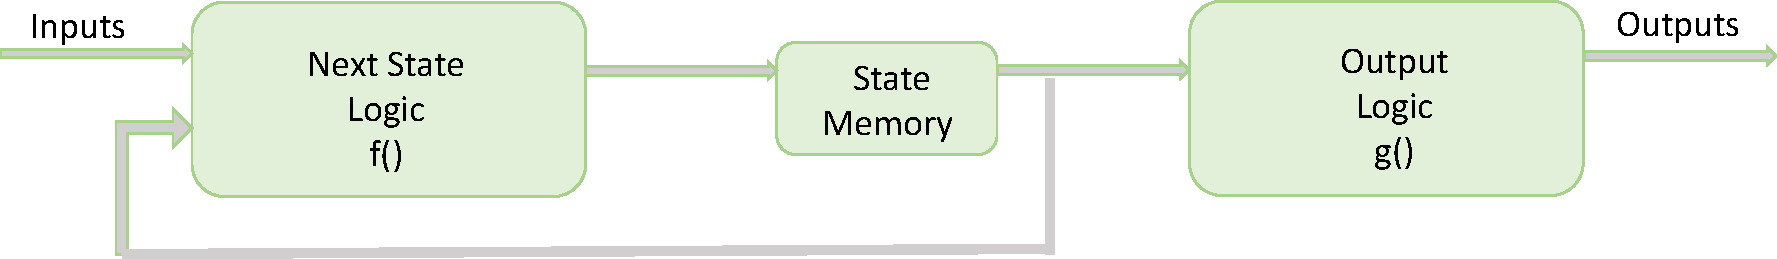
\includegraphics[width = 18cm]{./schema_FMG.pdf}
      \end{center}
  \end{figure}
  
 We define the next state with our transition function, we memorize the present state and generate the outputs and then we define the new next state with the present state and the new inputs.\\
 It's adapted to be implemented in different languages. Our project uses the language object Matlab implementation, where each class has a present State containing his intern situation and his own evolution functions $f()$, $m()$ and $g()$ that read the inputs, calculate outputs and the next State.






